\documentclass[conference]{IEEEtran}
\IEEEoverridecommandlockouts
% The preceding line is only needed to identify funding in the first footnote. If that is unneeded, please comment it out.
\DeclareFontShape{JT2}{mc}{m}{sc}{<->ssub*mc/m/n}{}
\usepackage{cite}
\usepackage{amsmath,amssymb,amsfonts}
\usepackage{algorithmic}
\usepackage{textcomp}
\usepackage{xcolor}
\usepackage{flushend}
\usepackage[dvipdfmx]{graphicx}
\def\BibTeX{{\rm B\kern-.05em{\sc i\kern-.025em b}\kern-.08em
    T\kern-.1667em\lower.7ex\hbox{E}\kern-.125emX}}
\begin{document}

\title{The New Fake News Detection with Generated Comments for News Article% *\\
% {\footnotesize \textsuperscript{*}Note: Sub-titles are not captured in Xplore and
% should not be used}
% \thanks{Identify applicable funding agency here. If none, delete this.}
}

\author{\IEEEauthorblockN{Yuta Yanagi}
\IEEEauthorblockA{\textit{Department of Informatics} \\
\textit{the University of Electro-Communications}\\
Tokyo, Japan \\
yanagi.yuta@ohsuga.lab.uec.ac.jp}
\and
\IEEEauthorblockN{Yasuyuki Tahara}
\IEEEauthorblockA{\textit{Department of Informatics} \\
\textit{the University of Electro-Communications}\\
Tokyo, Japan \\
tahara@uec.ac.jp}
\and
\IEEEauthorblockN{Yuichi Sei}
\IEEEauthorblockA{\textit{Department of Informatics} \\
\textit{the University of Electro-Communications}\\
Tokyo, Japan \\
sei@uec.ac.jp}
\and
\IEEEauthorblockN{Akihiko Ohsuga}
\IEEEauthorblockA{\textit{Department of Informatics} \\
\textit{the University of Electro-Communications}\\
Tokyo, Japan \\
ohsuga@uec.ac.jp}
}

\maketitle

\begin{abstract}
Recently, fake news spread via social networks and make the wrong rumor faster.
This problem is serious because the wrong rumor sometimes make social damage via deceived people.
Fact-checking is an ordinary solution to measure the credibility of news articles.
However this process usually takes a long time and it is hard to make it before spreading the wrong rumor.
Automatic detection of fake news is a popular researching topic.
It is confirmed that considering not only articles but also social context(i.e. likes, retweets, replies, comments, etc.) supports to spot fake news correctly by them.
This type is also hard to detect fake news before spreading the wrong rumor because social context is made with spreading on social networks.
We propose a fake news detector with generating part of the social context which is extended from the fake news generator model.
This model is trained about generating comments and classification of real/fake by dataset which is combined news and comments.
To measure this model's classification quality, we checked classification results from articles with real comments and generated ones by itself.
We compared results between classified with attached a generated comment and real comments only and we got results that considering a generated comment help detect more fake news than considering real comments only.
\end{abstract}

\begin{IEEEkeywords}
fake news, disinformation, neural network, natural language processing, deep-learning, microblogs
\end{IEEEkeywords}

\section{Introduction}
In this era, social media is one of the important parts of our lives.
Social media makes it easier to get news and share them with friends online.
However, at the same moment, 
there is also information that includes less credibility.
Some of them have obvious misinformation that is made by malicious purpose,
we call them ``fake news''.

Fake news try to make wrong rumors by spreading on social media.
This year, there is so much fake news about COVID-19 and sometimes these make wrong rumors online.
Directer of General of the WHO called this problem ``infodemic'' and he told that fake news spreads faster and more easily than itself\cite{ZAROCOSTAS2020676}. 
Besides, fake news created some mayhem not only online, but also offline (real incidents)
e.g. in Washington, fake news about the Pizzagate conspiracy is reported to have motivated the shooting\cite{agencies_2016}.
Spreading fake news also shakes the premise of democracy due to people cannot get accurate information.
Therefore, some researches try to spot fake news by machine learning.

The challenging point of this is there are news articles which try to deceive readers
and this makes it harder to classify by a simple rule-based method.
To get more information to detection,
there are some works which aggregate social context i.e. Retweet, Like, and comments
report better results than only considering news text\cite{Guo:2018:RDH:3269206.3271709}.
However, social contexts are not able to get before spreading.
Hence, there is also a work that generates words of comments from the news by CVAE to detect fake news when they are just posted\cite{ijcai2018-533}.
Their work tries to generate comments, but generated ones are only words that have a high probability of appearing.

In this work, we will propose a model that evaluates news credibility by news text and generated comments.
This model is modified from generating fake news articles\cite{NIPS2019_9106} and this model trains not only news features but also generating comments.
In training, this sequence includes real posted comments but the test sequence does not use them to simulate operation in real-social media.
The skill of generating comments help classification in the test sequence.

We measure the performance of our proposed method by some experiments with a real-posted dataset.

\section{Related works}
To detect and classify fake news is not a new topic because it is so similar to detecting spam\cite{shen2017discovering}, rumor\cite{7023340}, and illegal advertisement\cite{Huang:2017:DFO:3041021.3054233}.
Following some previous works\cite{Shu:2017:FND:3137597.3137600,Ruchansky:2017:CHD:3132847.3132877,Wang:2018:EEA:3219819.3219903}, we define fake news as news that is intentionally fabricated and can be verified as false.

\subsection{Detecting fake news}
There are many works which detect fake news with only news content.
In-text features, writing styles\cite{DBLP:journals/corr/PotthastKRBS17} and amount of emotions\cite{DBLP:journals/corr/abs-1903-01728}
were considered because commonly fake news has original styles and emotions.
Besides, using deep neural networks achieved better results in classification on some works\cite{wang-2017-liar,karimi-tang-2019-learning,karimi-etal-2018-multi}.

Many works consider the social context of news content.
The Social context feature is generated by user-based\cite{Castillo:2011:ICT:1963405.1963500,8397048,DBLP:journals/corr/abs-1904-13355}, 
post-based\cite{Yang2019UnsupervisedFN,Tacchini2017SomeLI,Jin:2016:NVE:3016100.3016318},
 and network-based\cite{Wu:2018:TFF:3159652.3159677,DBLP:journals/corr/abs-1902-06673}.

Considering the social context, it must wait for moments from posted because social contexts are made by users who are exposed.
Therefore, a Two-Level Convolutional Neural Network with User Response Generator(TCNN-URG) was proposed\cite{ijcai2018-533}.
This generates comment by hidden variables which are trained by a probable distribution of comment appearance.
Generating comments can give additional information to classify posts and get even if the news is just posted.
However, this generates only words that have a high probability of appearance and there are no grammar elements.

\subsection{Generating fake news}
\label{subsec:generate}
In generating natural language articles, the Grover model made so natural neural fake news articles\cite{NIPS2019_9106}.
This model is trained by news which separated into news domain, author, posted date, title, and article and evaluate the prediction.
The interesting thing is that human beings are more likely to be fooled by generated articles being real ones.
We tried to extend this model and generate naturally comments.
\section{methodology}
Like \ref{subsec:generate}, the original Grover model was trained by news which had five parts.
Each part is attached start and end token and some of them are dropped to predict.
We replaced the other part of the article to three comments and tried to predict one of the comments.
We modeled by the joint distribution alongside the original one:
\begin{equation}
    \label{eq:joint_distri}
    p = (\rm{article}, \rm{comment\_1}, \rm{comment\_2}, \rm{comment\_3})
    \end{equation}
The original one was made for generation of fake news but our proposed model was arranged to generate comments.

\begin{figure*}[!t]
    \centering
    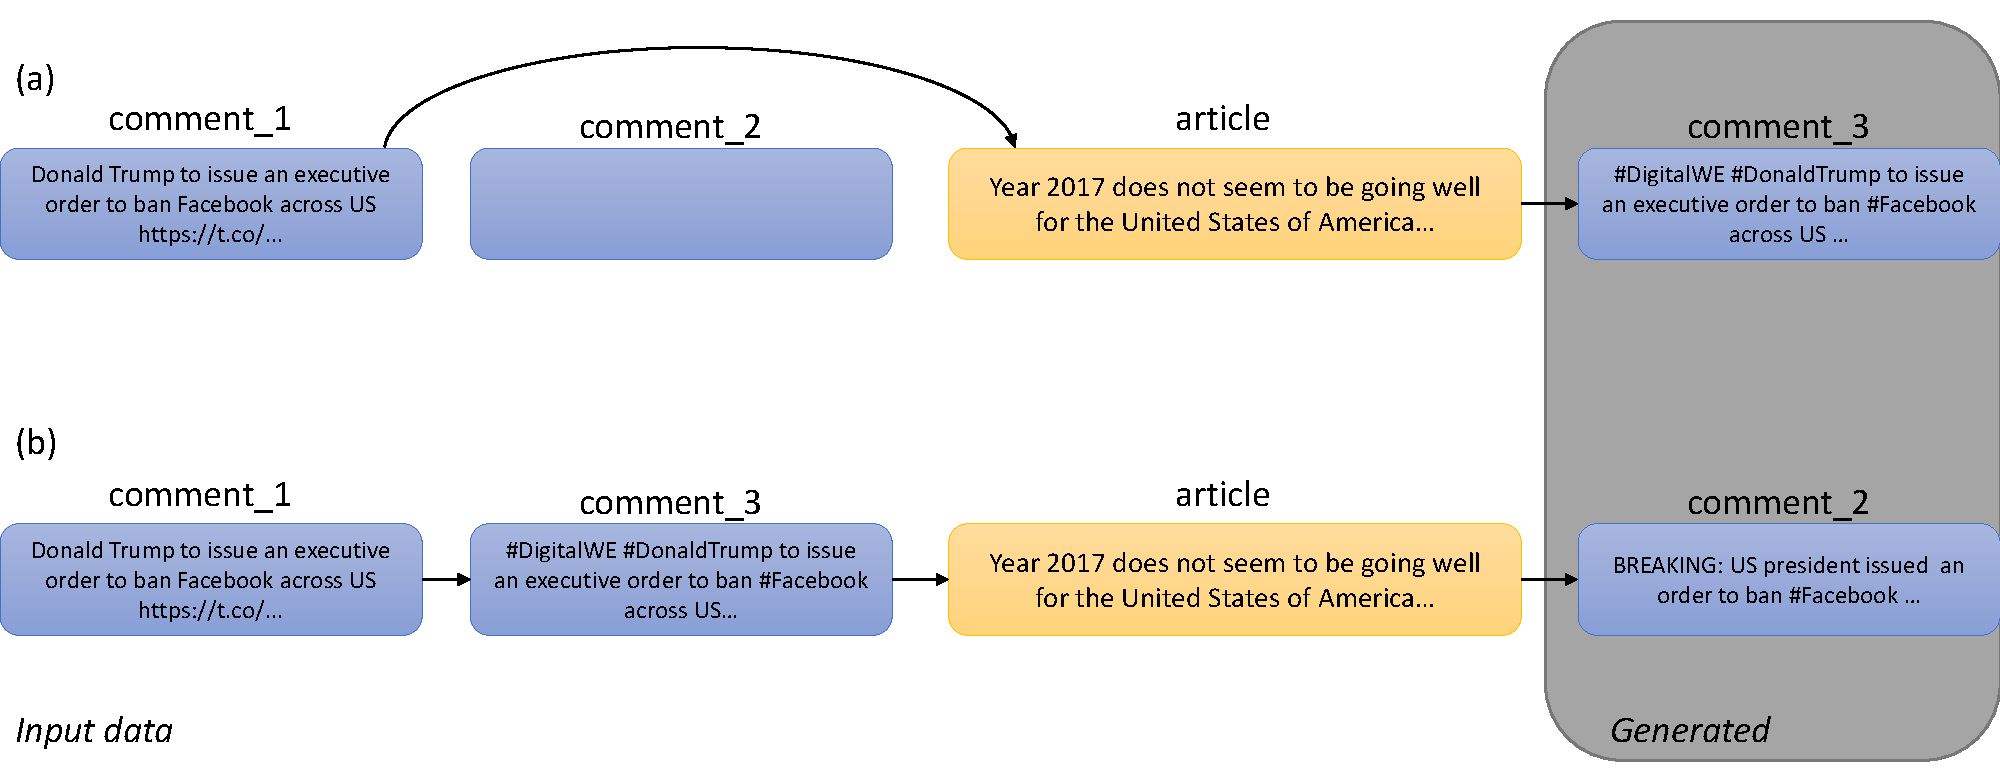
\includegraphics[width=\linewidth,pagebox=cropbox,clip]{fig_method.pdf}
    \caption{
        An ordinary diagram of two generations of our proposed method.
        (a) shows that one of the comments was generated from partly dropped contexts for comments.
        (b) shows that another one was generated from contexts that include a generated comment from (a).
    }
    \label{fig:method}
\end{figure*}
\section{results}
\subsection{Word generation tendency}
\label{subsec:trend}
First of all, we investigated the difference between generated comments from real and fake news.
We generated comments which refer to news articles that are fact-checked by PolitiFact from the FakeNewsNet dataset\cite{Shu2018FakeNewsNetAD}.
This dataset contains sets of a news article and tweets(comments) which refer to it.
We filtered news which have at least three tweets and sampled three tweets for generating.
Both real and fake labels have 200 sets of an article and comments and we trained to generate comments. 
We used these indexes: times of used words, percentage of used words, and the gap of a percentage point of used words of generated comments from real and fake.
We removed extra elements: stop words by NLTK, url(starts with \textit{http, https}), and part of symbols.
We didn't remove mentions, colons, and hashtags(i.e. @anyone, analyze: \#anything).
We found these features of all generated comments:
\begin{itemize}[\IEEEsetlabelwidth{3}]
    \item The most generated word was ``via''(c. 1.5\%).  
    \item ``via'' was also the top frequency of generated word from both real and fake. 
    \item The second and third were ``trump'' and ``obama'' but both their percentages were under 1\%.
    \item The generated comments seemed to be not accurate in grammar.
\end{itemize}
We also found the difference between generated comments from real and fake news.
\begin{itemize}[\IEEEsetlabelwidth{3}]
    \item The percent about the frequency of ``via'' in generated comments from fake news article was twice as much as ones from real news.
    \item ``via'' was also the most gap of frequency between generated comments from real and fake.  The delta was approx. 0.9 percentage point.
    \item ``breaking:'' was the second of the most percentage point between frequency(fake was more than real). the delta was approx. 0.7 percentage point.
\end{itemize}
\subsection{Quality of classify}
We measured the effect of generated comment for classification by comparing classification without a generated comment.
We prepared baselines: classify by only a news article, with two real-posted comments.
We used pairs of an article of GossipCop and tweets instead because ones of PolitiFact were too few to make classification accurate.
We sampled the same rule of \ref{subsec:trend} but both real and fake labels have 2000 sets.
The result of classification is Table \ref{tbl:classify_results}.
Our proposed method was best of recall s core but precision was worse than consider without generated comments.
\begin{table}[!t]
    \renewcommand{\arraystretch}{1.3}
    \caption{Results of classification}
    \label{tbl:classify_results}
    \centering
    \begin{tabular}{lccc}
    \hline
    Model name           & Precision & Recall & F1 score \\ \hline
    Article only         & 0.647     & 0.615  & 0.631    \\
     + Real comment * 2  & \textbf{0.682}     & 0.750  & \textbf{0.714}    \\
     + Generated comment & 0.590     & \textbf{0.790}  & 0.675    \\ \hline
    \end{tabular}
    \end{table}
\section{discussion}
\subsection{Generating comments}
According to trends of words in generated comments, our proposed method seemed to be trained by the credibility of news articles.
Most of the generated comments referred to topics of politics and this may be caused by the character of the dataset.

The interesting word of generated comment is ``breaking:''.
Our experiment results showed that this word is more generated by fake news than real news.
This phenomenon was also confirmed in the research of TCNN-URG\cite{ijcai2018-533}.

The quality of the grammar was clearly not as good as it should have been by human A/B testing.
This is caused by a lack of dataset scale. 
Grover article used 120 gigabytes of dataset\cite{NIPS2019_9106}.
We need to search or get a more large dataset of sets of articles and tweets.

\subsection{classification}
According to TABLE \ref{tbl:classify_results}, our proposed model made the best score of recall but precision was the worst score.
This means the proposed model can detect more fake news than another model which doesn't use generated comments even if social contexts are limited. 
The trend suggests that this model helps for people who search for news which are needed to fact-checking. 
However, the model also detected more not fake news than another one so this is a point of improvement.
We will check if the trend is changed by scale of dataset.
\subsection{Suggestions of improvements}
\appendix[Settings of experiments]
\label{app:settings}
\begin{itemize}[\IEEEsetlabelwidth{3}]
    \item Trained on Ubuntu 16.04 on Docker in Linux server with TITAN X (Pascal).
    \item Our proposed model was extended from grover repository by forking on GitHub.
    \item Model size was Grover-Base but we reduced vocabulary a little bit in order to fit for extension.
\end{itemize}
\bibliographystyle{IEEEtran}
\bibliography{IEEEabrv,myreferences}

\end{document}
